\chapter{Performantie}
\label{app:performantie}

In deze appendix wordt een gedetailleerd overzicht gegeven van de performantie voor de vier raamwerken op de acht apparaten: 
\st{} (zie \ref{app:performantie-st}),
\kendo{} (zie \ref{app:performantie-kendo}),
\jqm{} (zie \ref{app:performantie-jqm}),
\lungo{} (zie \ref{app:performantie-lungo}).

%%%%%%%%

\section*{\st}
\label{app:performantie-st}
\begin{figure}
  \centering
  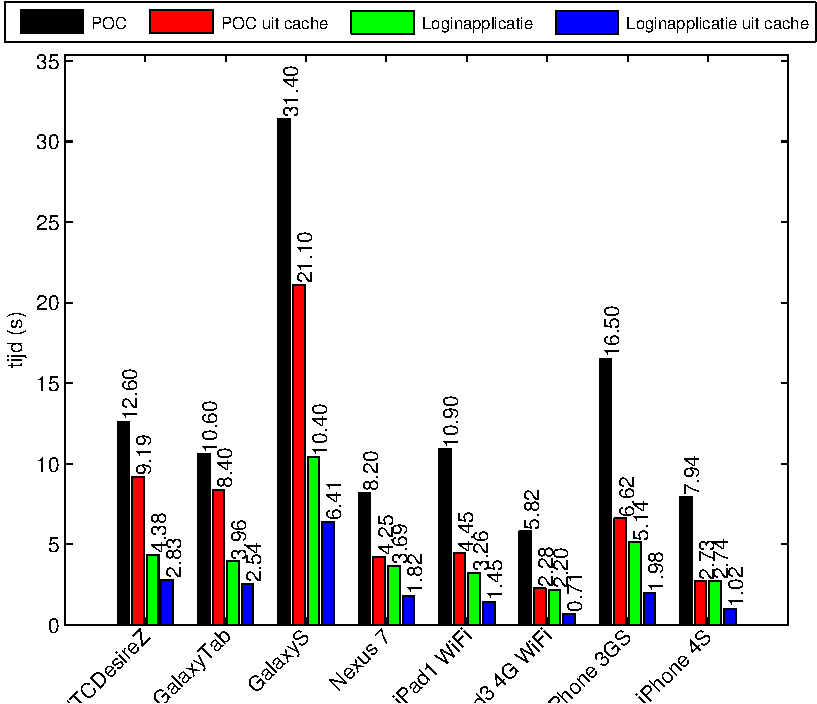
\includegraphics[width=0.75\textwidth]{figuren/performance-st.pdf}
  \caption{Gemiddelde downloadtijden van \st{} voor POC,  POC uit cache,  loginapplicatie en loginapplicatie uit cache voor elk apparaat.}
  \label{fig:performantie-st}
\end{figure}

Op figuur~\ref{fig:performantie-st} wordt de gemiddelde downloadtijd van \st{} getoond op elk apparaat.
Voor de POC is een dalende downloadtijd waarneembaar wanneer het Android-apparaat recenter wordt.
De downloadtijd van de POC op de \gs{} duurde gemiddeld $31.43\unit{s}$.
Gemiddeld moeten Android-toestellen $5\unit{s}$ langer laden in vergelijking met iOS-toestellen.
Dit gemiddelde wordt sterk beïnvloed door de trage downloadtijd van de \gs{}.

Een opmerking die bij \st{} moet worden gemaakt, is dat AJAX-verzoeken van een \code{Proxy} naar een ander domein altijd vooraf worden gegaan met een OPTIONS-verzoek.
Dit is een verzoek om informatie over de beschikbare opties van het communicatiekanaal op te vragen.
Standaard zet \st{} de \code{X-Requested-With} op XMLHttpRequest en hierdoor zal de browser een OPTIONS-verzoek als \term{preflight} sturen.

%Setting custom headers on XHR requests triggers a preflight request. %http://remysharp.com/2011/04/21/getting-cors-working/
%http://stackoverflow.com/questions/10236056/when-loading-a-store-in-sencha-touch-2-how-can-i-stop-the-additional-options-ht
% POST /resources/userService/login?_dc=1368367749599 HTTP/1.1
% Host: kulcapexpenseapp.appspot.com
% Connection: keep-alive
% Content-Length: 54
% Origin: http://sandervanloock.github.io
% User-Agent: Mozilla/5.0 (X11; Linux i686) AppleWebKit/537.11 (KHTML, like Gecko) Chrome/23.0.1271.64 Safari/537.11
% Content-Type: application/x-www-form-urlencoded; charset=UTF-8
% Accept: */*
% Referer: http://sandervanloock.github.io/HTMobieL/Sencha/build/ExpenseApp/production/index.html
% Accept-Encoding: gzip,deflate,sdch
% Accept-Language: nl-NL,nl;q=0.8,en-US;q=0.6,en;q=0.4
% Accept-Charset: ISO-8859-1,utf-8;q=0.7,*;q=0.3
% 
% Accept:*/*
% Accept-Charset:ISO-8859-1,utf-8;q=0.7,*;q=0.3
% Accept-Encoding:gzip,deflate,sdch
% Accept-Language:nl-NL,nl;q=0.8,en-US;q=0.6,en;q=0.4
% Connection:keep-alive
% Content-Length:23
% Content-Type:application/x-www-form-urlencoded; charset=UTF-8
% Host:kulcapexpenseapp.appspot.com
% Origin:http://sandervanloock.github.io
% Referer:http://sandervanloock.github.io/HTMobieL/Sencha/build/ExpenseApp/production/index.html
% User-Agent:Mozilla/5.0 (X11; Linux i686) AppleWebKit/537.11 (KHTML, like Gecko) Chrome/23.0.1271.64 Safari/537.11
% X-Requested-With:XMLHttpRequest

%%%%%%%%

\section*{\kendo}
\label{app:performantie-kendo}

\begin{figure}
  \centering
  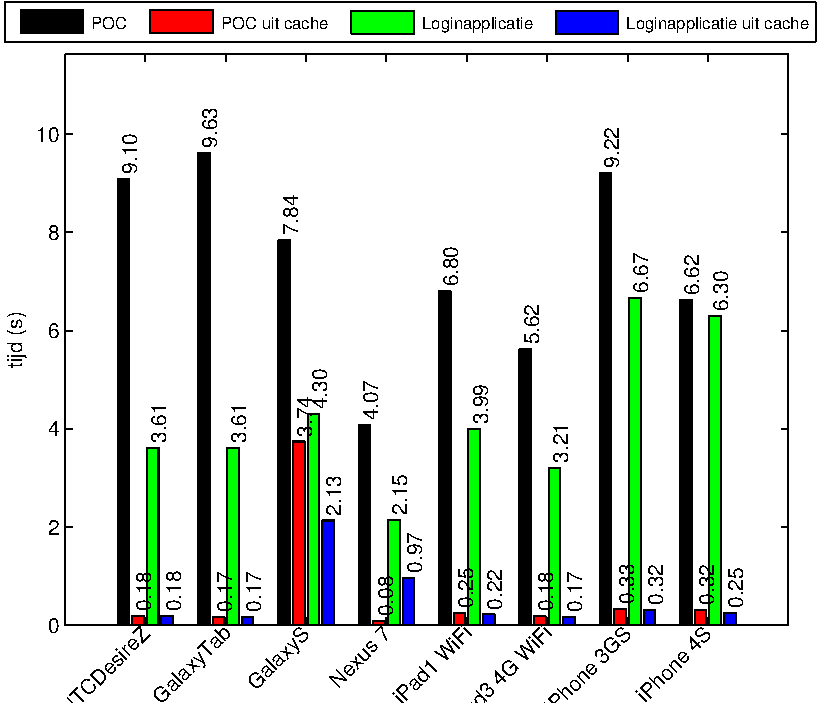
\includegraphics[width=0.75\textwidth]{figuren/performance-kendo.pdf}
  \caption{Gemiddelde downloadtijden van \kendo{} voor POC,  POC uit cache,  loginapplicatie en loginapplicatie uit cache voor elk apparaat.}
  \label{fig:performantie-kendo}
\end{figure}

Op figuur~\ref{fig:performantie-kendo} worden de gemiddelde downloadtijd van \kendo{} getoond op elk apparaat.
De \gtab{} vertoont de hoogste downloadtijd,  gevolgd door de \iphoneiii{} en \htc.
Opmerkelijk is dat de loginapplicatie uit cache op de \nexus{} tien keer trager laadt dan de POC uit cache.
Het ophalen van een applicatie uit cache werkt bij de \gs{} het traagst.
Bij \kendo{} is er geen opmerkelijk verschil waarneembaar tussen Android- en iOS-toestellen.
Android is gemiddeld $60\unit{ms}$ trager.

%%%%%%%%

\section*{\jqm}
\label{app:performantie-jqm}

\begin{figure}
  \centering
  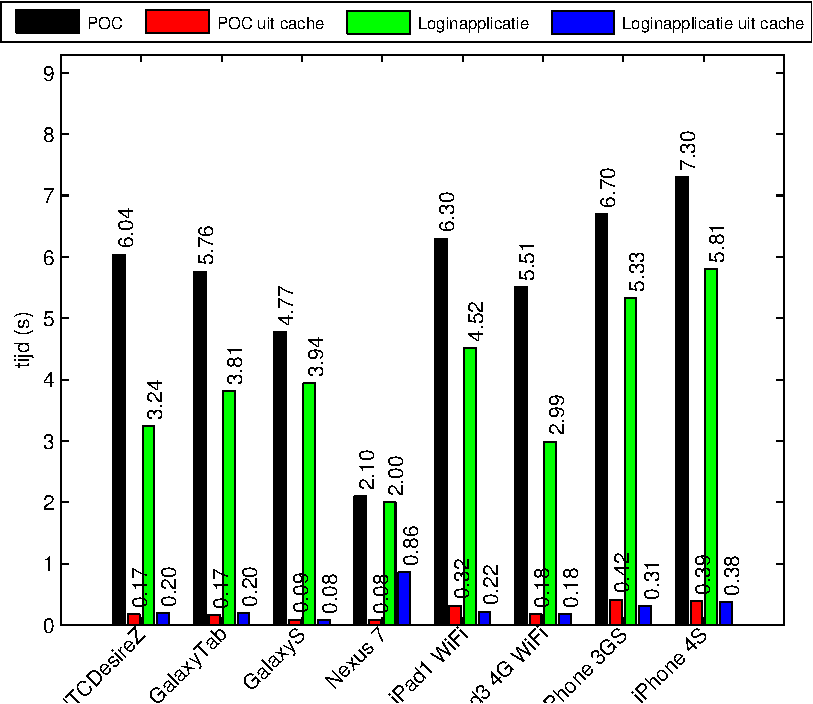
\includegraphics[width=0.75\textwidth]{figuren/performance-jquery.pdf}
  \caption{Gemiddelde downloadtijd van \jqm{} voor POC,  POC uit cache, loginapplicatie en loginapplicatie uit cache voor elk apparaat.}
  \label{fig:performantie-jqm}
\end{figure}

Op figuur~\ref{fig:performantie-jqm} wordt de gemiddelde downloadtijd van \jqm{} getoond op elk apparaat.
Voor de POC is een dalende downloadtijd waarneembaar wanneer de Android-versies op het apparaat recenter worden.
iPads dalen in downloadtijd als het apparaat recenter wordt, daarentegen stijgt de downloadtijd bij iPhones.

Als de loginapplicatie wordt bekeken, wordt hetzelfde waargenomen als voor de POC.
Enkel bij de Android-apparaten wordt de downloadtijd trager, naarmate de Android-versie recenter wordt, wat in tegenstelling is tot de POC.
Enkel de \nexus{} volgt deze trend niet.
Op de \nexus{} wordt de loginapplicatie ongeveer even snel gedownload als de POC.
Een opmerkelijke waarneming is dat het op de \nexus{} langer duurt om de loginapplicatie uit cache te laden dan de volledige POC uit cache.

%%%%%%%%

\section*{\lungo}
\label{app:performantie-lungo}

Op figuur~\ref{fig:performantie-lungo} wordt de gemiddelde downloadtijd van \lungo{} getoond op elk apparaat.
Er is geen opmerkelijke trend waarneembaar voor Android.
Wel is er een opmerkelijke waarneming op de \gs{}, waarbij de downloadtijden uit cache langer duren dan $1\unit{s}$, terwijl op alle apparaten deze tijden rond de $0,25\unit{s}$ liggen.
Bij iOS daalt de downloadtijd als het toestel recenter is.
Zo is de downloadtijd op \ipadiii{} sneller dan \ipadi{}.
Het geldt ook zo dat de \iphoneiv{} sneller downloadt dan de \iphoneiii{}.

\begin{figure}[H]
  \centering
  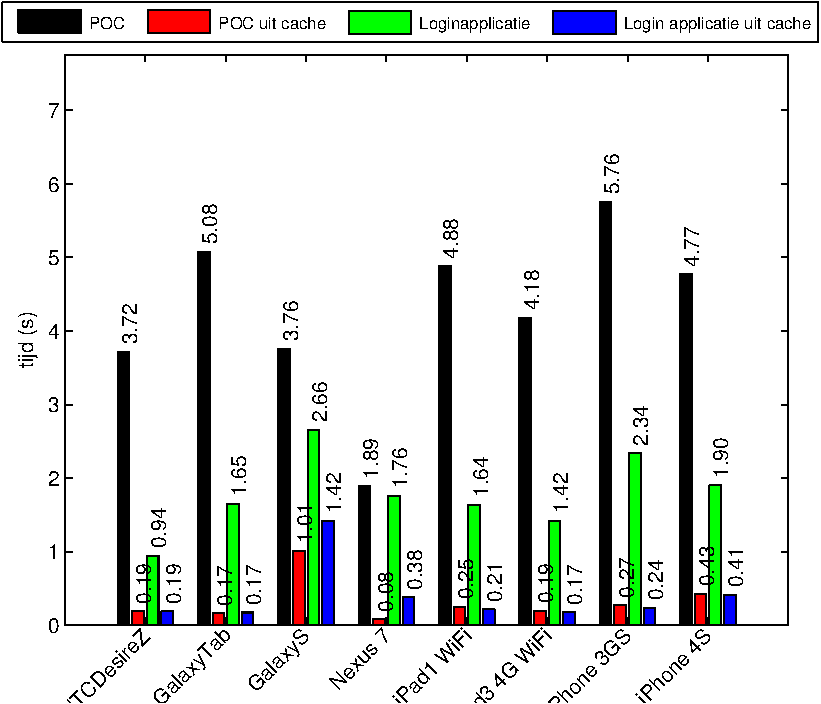
\includegraphics[width=0.75\textwidth]{figuren/performance-lungo.pdf}
  \caption{Gemiddelde downloadtijd van \lungo{} voor POC,  POC uit cache,  loginapplicatie en loginapplicatie uit cache voor elk apparaat.}
  \label{fig:performantie-lungo}
\end{figure}

%%% Local Variables: 
%%% mode: latex
%%% TeX-master: "masterproef"
%%% End: 
